\section{Recent Research Progress}
\sheading{Chromatin organization and DNA replication in \scer}
\ssheading{Chromatin architecture of replication origins}
To better understand how the chromatin environment impacts the selection and regulation of replication origins across the genome, we simultaneously evaluated the DNA occupancy of nucleosomes and the majority of DNA-binding proteins (\eg transcription factors and replication initiation proteins) to generate genome-wide chromatin occupancy profiles (GCOPs)({\color{dukeblue}\textbf{Figure 2}}). Briefly, total chromatin is digested with micrococcal nuclease (MNase) and all of the recovered DNA fragments are subjected to paired-end next-generation sequencing\citep{Belsky2015-li,Henikoff2011-vo}.  Importantly, the size of the sequenced fragment represents whether it was protected by a nucleosome ($\sim$147 bp) or a DNA-binding factor ($<$50 bp). This assay is factor agnostic and reveals specific footprints for more than 70\% of the yeast DNA-binding factors\citep{Henikoff2011-vo}.  Although, the assay only provides information about the occupancy state of the DNA, we can often infer the identity of the factor bound from motifs and prior genomic experiments.  
\begin{floatingfigure}[lt]{2.5in}
\vspace{-8mm}
\begin{center}
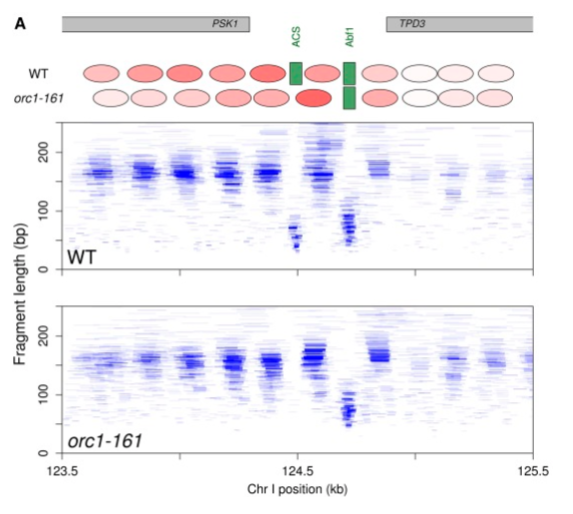
\includegraphics[width=2.5in]{r35_figures/orc_chromatin.png}
\end{center}
\vspace{3mm}
\caption{Genome-wide chromatin occupancy footprint (GCOP) of a replication origin.  Protected DNA fragments were recovered from an MNase digestion and subject to paired-end sequencing. Fragment length is plotted as a function of chromosomal position.  Well phased fragments at $\sim$150 bp represent sequences protected by nucleosomes and smaller fragments represent other DNA binding factor footprints.  In a temperature sensitive \textit{ORC1-161} mutant the footprint at the ACS disapears at the non-permissive temperature.}%
\end{floatingfigure}%
Our `footprinting' of the \scer genome at distinct cell cycle stages provided the  %the We `footprinted' the \scer\ genome at multiple points in the cell cycle including G2 (ORC alone) and G1 (pre-RC assembly)\citep{Belsky2015-li}.  Together, these experiments provide the 
following advances and new insights into our understanding of the DNA replication program: i) a novel method to map origins of DNA replication by their ORC-dependent chromatin footprints -- this data provides structural information not only about ORC binding but also the surrounding chromatin and adjacent DNA binding factors at each individual origin; ii) we identified a non-canonical class of inefficient origins that lacked an ORC-dependent footprint in G2, but exhibited a clear footprint in G1 -- the mechanistic implication being that determinants of replication efficiency are established in G2 prior to pre-RC assembly; iii) nucleosome remodeling at the origin is required for efficient origin activation, but not pre-RC assembly -- highlighting the importance of nucleosome dynamics for downstream initiation events including origin unwinding and activation; iv) one Mcm2-7 double hexamer is loaded per origin in complex with either the up or downstream flanking nucleosome -- addressing a fundamental question in the field -- where, in relation to ORC, and how many Mcm2-7 double-hexamers are loaded per origin \invivo. 


%Start sites of DNA replication in \scer are defined by both cis- and trans-acting factors.  The  ACS (ARS consensus sequence) is a T-rich degenerate motif that occurs more than 10,000 times throughout the yeast genome\cite{}.  Despite the prevalence of high quality sequence matches to the ACS, fewer than 300 function as origins of DNA replication or interact with ORC\citep{}.  The specificity of ORC for only select ACS sites throughout the genome is likely mediated by the local chromatin structure.  In collaboration with Steve Henikoff, we have pioneered a micrococcal nuclease-based assay to 'footprint' the entire yeast genome at nucleotide resolution.

%cautionary tale about mnase
%need to integrate with introduction

%\ssheading{Mcm2-7 loading is limited by chromatin architecture}


Recent work in the laboratory has sought to identify the ATP-dependent chromatin remodeling activities responsible for nucleosome dynamics at replication origins.  %We have systematically evaluated all single, double and triple combinations of non-essential chromatin ATP-dependent chromatin remodelers in \scer for their impact on ORC binding, pre-RC assembly and origin activity. While the replication program was surprisingly resistant to loss of ATP-dependent chromatin remodelers, 
We found that both \textit{ISW1} and \textit{CHD1} activity were required for origin activation of late inefficient origins (manuscript submitted). In collaboration with Steve Bell, we have recently demonstrated that the \invitro assembly of nucleosomes by specific chromatin remodeling enzymes can impact pre-RC assembly and initiation in a reconstituted system\citep{Azmi2017-gg}.

%key steps We have also enjoyed a fruitful collaboration with Stephen P. Bell at MIT by which we have been able to apply the respective strengths of our laboratories (genomics and biochemistry) to fully explore specific hypotheses \invitro and \invivo.  Most recently we have demonstrated that nucleosome organization and phasing by specific ATP-dependent chromatin remodelers is important for pre-RC assembly and activation \invitro\citep{Azmi2017-gg}. 

%\ssheading{Mcm2-7 loading is limited by chromatin architecture}
%\begin{floatingfigure}[r]{2.1in}
%\vspace{-8mm}
%\begin{center}
%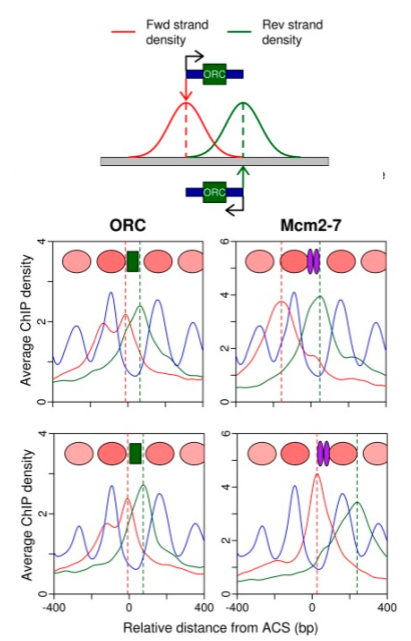
\includegraphics[width=2.1in]{r35_figures/mcm_histone.png}
%\end{center}
%\vspace{3mm}
%\caption{Pre-RC assembly at replication origins in the context of chromatin. The Mcm2-7 complex is loaded onto origins by ORC, Cdc6 and Cdt1 through multiple rounds of ATP hydrolysis\citep{BRC+04,RBR+06}. Nucleosome positioning and chromatin remodeling are conserved features of the eukaryotic DNA replication program\citep{Ding:2011uq}.}%
%\end{floatingfigure}%
%During G1, a cascade of ORC-dependent biochemical events occur at origins of replication culminating in the loading of the Mcm2-7 double-hexamer. 
%Although well-characterized on template DNA \invitro\citep{Randell2006-ln}, the mechanics of pre-RC formation remains elusive within the diverse chromatin environments surrounding replication origins \invivo.  Despite assembling the same proteins, different replication initiation sites vary substantially in both their activation time and efficiency\citep{Bechhoefer2012-bf}. Origin activation and efficiency are thought, in part, to be determined by rate limiting replication initiation factors in S-phase\citep{Mantiero2011-me}, chromatin modification state\citep{Knott2012-mp,Knott2009-vr,Vogelauer2002-pm}, and by the number of Mcm2-7 loaded at each origin\citep{Das2015-dz}. 

%We found that the local chromatin architecture is an important determinant of origin efficiency.   and  that  efficiency is that Mcm2-7 loading is limited by the local chromatin structure to one Mcm2-7 double-hexamer per origin\citep{Belsky2015-li} and that efficiency may be  . 


%While prior estimates of Mcm2-7 loading were based  on the total ChIP-seq signal emanating from each origin, we instead focused on the position of the Mcm2-7 ChIP-signal relative to the origin.  Unlike ORC whose ChIP-seq signal was centered on the ACS in the nucleosome free region, we found that the Mcm2-7 ChIP-seq signal coincided with either the up or downstream flanking nucleosome.  Examination of the chromatin fragments at nucleotide resolution demonstrated that the widths of the ChIP-seq signal corresponded to almost exactly the expected width of a nucleosome and a double hexamer of the Mcm2-7 complex.  Understanding the significance and the mechanism by which the Mcm2-7 complex associates with either the up or down stream nucleosome is an important question going forward.


%-- addresses a fundamental question in the DNA replication field -- where, in relation to ORC, and how many Mcm2-7 double-hexamers are loaded per origin \invivo. 
%In contrast, the distribution of fragment sizes in the ORC or Abf1 ChIP-seq experiments from the same were significanlty tigher.


%Resolution of the sheared immunoprecipiated chromatin fragments fWe found that the Mcm2-7 was in complex with either the up- or downstream-nucleosome flanking the origin of DNA replication and that the width of the ChIP-seq signal corresponded to almost exactly the expected width of a nucleosome and a double hexamer of the Mcm2-7 complex..  


%The data are clear and not seen with Abf1 or ORC. Understanding the signficance of this association and the mechanism -- is of importance.  can try moving nucleosome  

%One model to account for this is the rhind model. 





%Although well-characterized on template DNA \invitro, pre-RC formation remains elusive within the diverse chromatin environments surrounding replication origins \invivo.  Despite assembling the same proteins, different replication initiation sites vary substantially in both their activation time and efficiency.  One model to account for this is the rhind model.  We originally sought to identify sites of pre-RC assembly by our MNase footprinting assay, but the Mcm2-7 complex appears to translocate off the DNA in the absence of robust cross linking.  Instead, we examined the distribution of Mcm2-7 relative to the ACS and ORC binding.  If an origin of replication had multiple Mcm2-7 complexes loader per origin we would expect spreading -- or altivernatiely -- only one peak.  We found that Mcm





%The Mcm2-7 double hexamer is loaded in two steps onto origin DNA.  Reitterative loading.  We found that the Mcm2-7 complex is loaded asymmetrically surrounding ORC binding sites in the yeast genome. Start with Abf1, ORC and then MCM2-7  Specifcally, we found that Mcm2-7 was in complex with either the up- or downstream-nucleosome flanking the origin of DNA replication.  The data are clear and not seen with Abf1 or ORC. Understanding the signficance of this association and the mechanism -- is of importance.  can try moving nucleosome



\sheading{Establishment of the replication program and maintenance of genome integrity in \dros}
As a data production center for the model organism ENCODE (modENCODE) project we generated more than one hundred genome-wide datasets describing the replication timing, ORC localization and origin utilization in multiple \dros cell lines and tissues\citep{Mod_Encode_Consortium2010-io}.  In the capstone manuscript for the modENCODE project, more than 1400 genomic datasets from modENCODE and ENCODE revealed conserved principles and features of chromatin organization between flies, worms and humans\citep{Ho2014-xa}. %We identified conserved features of chromatin state and genome organization that were linked to the establishment of the DNA replication program. 
In addition to the capstone manuscript, we published 12 manuscripts over the course of the project. Below I've highlighted several of our mechanistic followup studies in \dros that were supported by our NIGMS R01.

\ssheading{DNA replication and transcription programs respond to the same epigenetic cues}
%The a time at which a sequence replicates during S-phase has long been coordinated with transcriptional activity in higher eukaryotes. 
We and others have correlated gene expression, open chromatin and chromatin modifications with origin location and replication timing data.  However, correlation does not  imply causation and due to multiple activating and repressive chromatin modifications it has been difficult to mechanistically assign a direct role to specific chromatin modifications in regulating the DNA replication program. We  demonstrated that the early replication of the \dros male X chromosome was dependent on dosage compensation and the male-specific H4K16 hyperacetylation of the X chromosome\citep{Lubelsky2014-zn}.  These results demonstrate that the transcription and DNA replication programs can respond to the same epigenetic cues.


%In the course of our modENCODE replication studies, we rediscovered that the male X chromosome replicates earlier than the autosomal chromosomes; I emphasize rediscover because early radiographic chromosome labeling experiments had previously noted that the male X-chromosome was early replicating.  The differential replication of the X chromosome relative to the autosomes only occurred in male cell lines suggesting that dosage compensation may be involved.  In Drosophila, sex chromosome dosage compensation is mediated by the Dosage Compensation Complex and the histone acetyltransferase, MOF, which hyperacetylates H4K16 specifically on the male X chromosome to up-regulate transcription two-fold.  We found that the early replication of the X-chromosome was dependent on the DCC and MOF in males and that over expression of msl2 was sufficient to promote eary replication in female cells.  


\ssheading{H4K20 monomethylation and genome integrity}
PR-Set7 is a cell cycle regulated methyl transferase that specifically monomethylates H4K20\citep{Beck2012-uc}.  In mammalian cells, loss of PR-Set7 and the resulting H4K20me1 is associated with delayed S-phase progression and elevated DNA damage presumably due to defects in pre-RC assembly and origin activation\citep{Tardat2010-qc}.  %However, prior studies only examined a handful of mammalian origins and it remained possible that the observed origin specific phenotypes were not due to perturbation of histone methylation, but PR-Set7 mediated methylation of other cell cycle  factors\citep{Shi2007-gz}. 
Although PR-Set7 is an essential gene in \dros, alanine substitution histone tail mutants (H4K20A) were sick but viable\citep{McKay2015-nn}, arguing that H4K20 methylation is not essential for DNA replication. We found that deregulation of PR-Set7 activity did not impact origin activation in \dros, but rather H4K20 mono-methylation was required for maintaining genomic integrity of late replicating domains\citep{Li2016-fi}.    


\ssheading{Mcm2-7 Paradox}
The `MCM Paradox' describes a %long standing 
series of %seemingly
paradoxical observations regarding the quantity and location of the replicative Mcm2-7 helicase complex during S-phase in higher eukaryotes\citep{Takahashi2005-bz}. Briefly, there is a vast excess of the Mcm2-7 complexes relative to origins of replication or ORC binding sites, the majority of which are %; %the Mcm2-7 complexes do not appear to localize to ORC by immunofluorescence experiments
%and the vast majority of the Mcm2-7 complex are 
dispensable during an unperturbed S-phase. We examined the `MCM Paradox'  using  genomic and biochemical approaches  to understand the mechanisms by which excess Mcm2-7 are loaded and distributed throughout the genome to preserve genomic integrity\citep{Powell2015-af}.  We found that during G1, Mcm2-7 is loaded onto chromatin in two distinct phases -- both of which rely on the canonical pre-RC assembly pathway including Dup/Cdt1 and Cdc6.  In the first phase of pre-RC assembly, a minimal level of Mcm2-7 is loaded specifically at ORC binding sites throughout the genome in a CDK independent manner.  There is also a second wave of pre-RC assembly that is CDK dependent which is required for the loading of the full complement (40 fold increase) of Mcm2-7 onto chromatin.  Strikingly, the full complement of Mcm2-7 is not restricted to sequences immediately adjacent to ORC binding sites, but rather distributed throughout the genome and shaped by active transcription.  %We find that the full complement of Mcm2-7 complex is displaced from actively transcribed regions suggesting that transcription can push or displace the Mcm2-7 complex through gene bodies.  
%Recent work from the Remus laboratory in \scer  has demonstrated that the Mcm2-7 complex can be pushed away from ORC binding sites by RNA Polymerase \invitro and \invivo resulting in origin activation being displaced from the site of pre-RC assembly\citep{Gros2015-oo}.  Together, 
These data provide an intriguing model whereby the transcription program may shape the distribution of the Mcm2-7 complex and ultimately origin location which may explain the seemingly random distribution of metazoan origins in higher eukaryotes\citep{Petryk2016-rr}.

